\section{Manutenzione}

\subsection{Aggiunta e aggiornamento librerie}

L'elenco delle librerie è presente nella cartella di root del progetto, nel file: "\textit{requirements.txt}".

\begin{figure}[H]
    \centering
    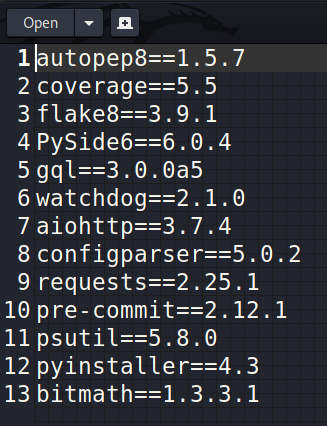
\includegraphics[scale = 0.5]{components/img/requirements.png}
    \caption{Struttura del file contenente le librerie}
    \label{fig:Struttura del file contentente le librerie}
\end{figure}
Per poter installare una nuova libreria il procedimento è semplice:
\begin{itemize}
	\item Aprire il file "\textit{requirements.txt}";
	\item Posizionarsi a fine file;
	\item Aggiungere una nuova riga;
	\item Aggiungere la nuova libreria.
\end{itemize}
La sintassi per l'aggiunta della libreria è la seguente:
\newline{} \centerline{\textbf{nome\_libreria==numero\_versione}}\newline{} 
\subsection{Struttura progetto}
Il progetto segue la seguente struttura:
\begin{figure}[H]
    \centering
    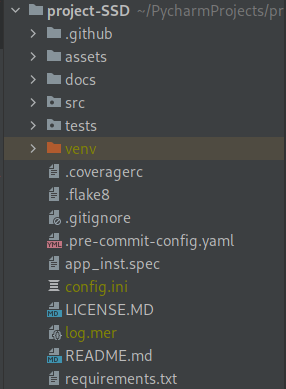
\includegraphics[scale = 0.5]{components/img/struttura-cartella-ssd.png}
    \caption{Struttura del progetto}
    \label{fig:Struttura del progetto}
\end{figure}  
\subsubsection{.github}    
\begin{figure}[H]
    \centering
    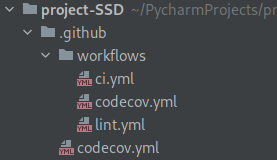
\includegraphics[scale = 0.5]{components/img/struttura-cartella-dotgithub.png}
    \caption{Struttura della cartella .github}
    \label{fig:Struttura della cartella .github}
\end{figure}    
\subsubsection{assets}    
\begin{figure}[H]
    \centering
    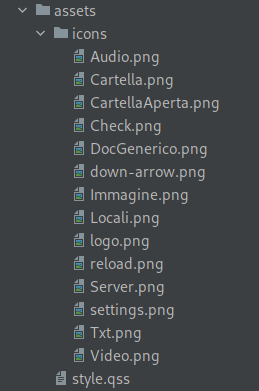
\includegraphics[scale = 0.5]{components/img/struttura-cartella-assets.png}
    \caption{Struttura della cartella assets}
    \label{fig:Struttura della cartella assets}
\end{figure}   
\subsubsection{docs}    
\begin{figure}[H]
    \centering
    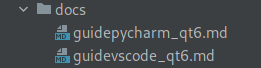
\includegraphics[scale = 0.5]{components/img/struttura-cartella-docs.png}
    \caption{Struttura della cartella docs}
    \label{fig:Struttura della cartella docs}
\end{figure}    
\subsubsection{src}    
\begin{figure}[H]
    \centering
    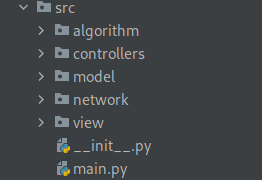
\includegraphics[scale = 0.5]{components/img/struttura-cartella-src.png}
    \caption{Struttura della cartella src}
    \label{fig:Struttura della cartella src}
\end{figure}    
\subsubsection{tests}    
\begin{figure}[H]
    \centering
    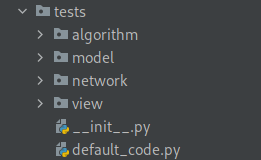
\includegraphics[scale = 0.5]{components/img/struttura-cartella-tests.png}
    \caption{Struttura della cartella tests}
    \label{fig:Struttura della cartella tests}
\end{figure}